\documentclass{ctexart}
\usepackage{graphicx}
\title{加法器实验}
\author{张明昆 2211585}
\date{2024.3.27}

\begin{document}
\maketitle
\tableofcontents
\section{实验目的}
1. 熟悉 LS-CPU-EXB-002 实验箱和软件平台。

2. 掌握利用该实验箱各项功能开发组成原理和体系结构实验的方法。

3. 理解并掌握加法器的原理和设计。

4. 熟悉并运用 verilog 语言进行电路设计。

5. 为后续设计 cpu 的实验打下基础。

\section{实验内容说明}
\subsection{实验设备}
1. 装有 Xilinx Vivado 的计算机一台。

2. LS-CPU-EXB-002 教学系统实验箱一套。
\subsection{实验任务}
1. 阅读 LS-CPU-EXB-002 实验箱相关文档,熟悉硬件平台。

2. 熟悉计算机中加法器的原理。

3. 画出结构框图,详细标出输入输出端口。

4. 根据设计的实验方案,使用 verilog 编写相应代码。

5. 对编写的代码进行仿真,得到正确的波形图。

6. 将以上设计作为一个单独的模块,设计一个外围模块去调用该模块,见图2.1。外围模块中需调用封装好的触摸屏模块,显示两个加数和加法结果,且需要利用触摸功能输入两个加数。

7. 将编写的代码进行综合布局布线,并下载到实验箱中的FPGA 板上进行演示。
\section{实验原理图}
\begin{figure}[ht]
    \centering
    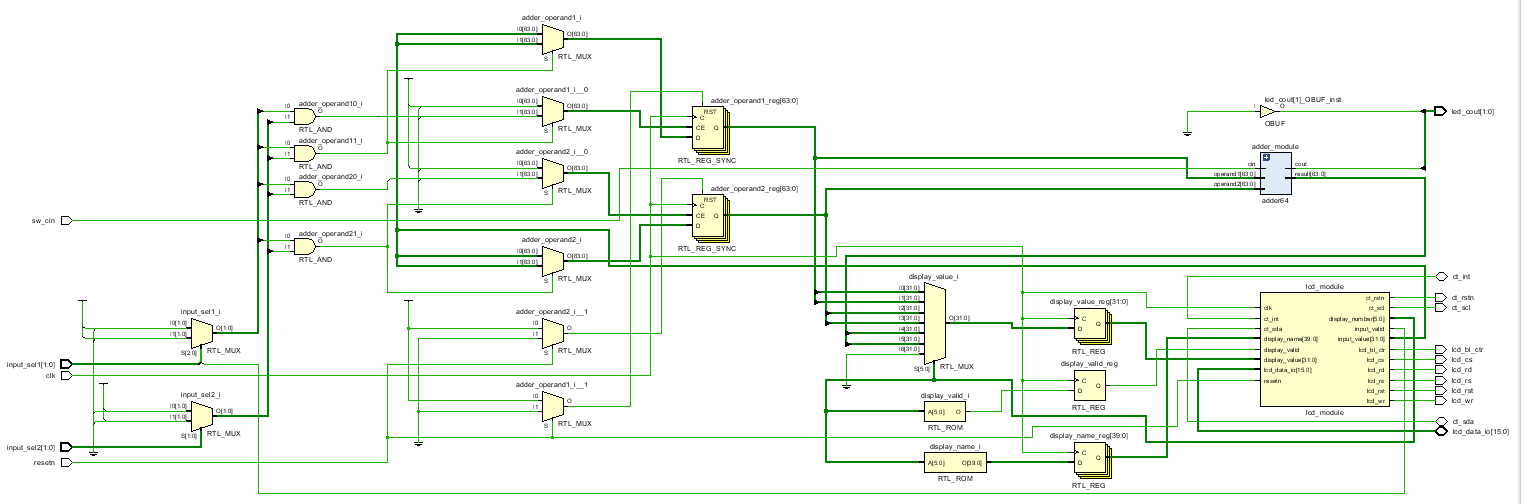
\includegraphics[width=1\textwidth]{./figures/schematic_diagram.png}
    \caption{实验原理图}
    \label{schematic_diagram}
\end{figure}
如图\ref{schematic_diagram}所示,adder\_display为该实验的顶层模块,其下有负责加法运算的adder64模块、负责显示控制的lcd\_module模块。

adder64模块执行两个64位数的加法运算。它接收两个64位的输入操作数 operand1 和 operand2,以及一个进位输入 cin。
通过对这两个操作数和进位进行加法运算,产生64位的结果 result 和一个进位输出 cout。加法运算采用了Verilog的加法操作符+实现。

lcd\_module模块负责控制LCD触摸屏的显示和输入。它通过一系列接口与触摸屏通信,包括显示有效信号 display\_valid、要显示的名称 display\_name、要显示的值 display\_value,以及控制触摸屏硬件接口的信号。
此模块也处理来自触摸屏的输入,包括有效输入信号 input\_valid 和输入值 input\_value。

adder\_display模块将加法器模块和显示控制模块连接起来,并管理它们之间的数据交互。它根据用户通过触摸屏输入的选择(通过 input\_sel 和 sw\_cin 控制),决定如何处理加法操作数和进位输入。
此外,它还控制LED(通过 led\_cout 输出)来显示加法操作的进位输出。此模块还处理触摸屏显示的逻辑,根据显示编号 display\_number 显示不同的数据。
\section{实验步骤}
\subsection{编写verilog代码}
为了实现题目中要求的64位加法器,我们需要实现一个64位的加法器如下所示。
\begin{verbatim}
    `timescale 1ns / 1ps
    module adder64(
        input  [63:0] operand1,
        input  [63:0] operand2,
        input         cin,
        output [63:0] result,
        output        cout
        );
        assign {cout,result} = operand1 + operand2 + cin;
    endmodule
    }
\end{verbatim}
为了使得其他模块能够与该加法器协同工作,我们需要对adde\_dispaly进行以下修改,每次输入一个数字的32位,分四次完成输入。
\begin{verbatim}
    //此处代码与指导手册相同,故不再列出
    input [1:0]input_sel1, //0:输入为加数1;1:输入为加数2
    input [1:0]input_sel2, //0:输入为低32位;1:输入为高32位
    //此处代码与指导手册相同,故不再列出
    always @(posedge clk)
    begin
        if (!resetn)
        begin
            adder_operand1 <= 32'd0;
        end
        else if (input_valid && input_sel1==0 && input_sel2 == 0)
        begin
            adder_operand1[31:0] <= input_value;
        end
         else if (input_valid && input_sel1==0 && input_sel2 == 1)
        begin
            adder_operand1[63:32] <= input_value;
        end
    end
    always @(posedge clk)
    begin
        if (!resetn)
        begin
            adder_operand2 <= 32'd0;
        end
        else if (input_valid && input_sel1==1 && input_sel2 == 0)
        begin
            adder_operand2[31:0] <= input_value;
        end
         else if (input_valid && input_sel1==1 && input_sel2 == 1)
        begin
            adder_operand2[63:32] <= input_value;
        end
    end
    //此处代码与指导手册相同,故不再列出
\end{verbatim}
\subsection{仿真验证}
书写仿真文件如下所示。
在initial块中,所有的输入寄存器(包括两个操作数的高低部分和进位输入)最初被设置为0。接着,在仿真开始后的100纳秒处,添加测试激励。

为了测试adder64在不同输入条件下的行为,该测试模块使用always块在每10纳秒生成随机数来更新操作数的高低部分和进位输入cin。
\begin{verbatim}
    module adder64_test;
    reg [31:0] operand1_low;
    reg [31:0] operand2_low;
    reg [31:0] operand1_high;
    reg [31:0] operand2_high;
    reg cin;
    wire [63:0] result;
    wire cout;
    // Instantiate the Unit Under Test (UUT)
    adder64 uut (
    .operand1({operand1_high, operand1_low}), 
    .operand2({operand2_high, operand2_low}), 
    .cin(cin), 
    .result(result), 
    .cout(cout)
);
    initial begin
        operand1_low=0;
        operand1_high=0;
        operand2_low=0;
        operand2_high=0;
        #100;
    end
    always #10 operand1_low = $random;
    always #10 operand1_high= $random;
    always #10 operand2_low = $random;
    always #10 operand2_high= $random;
    always #10 cin = {$random} % 2;
endmodule
\end{verbatim}

仿真波形图如图\ref{wave}所示
\begin{figure}[ht]
    \centering
    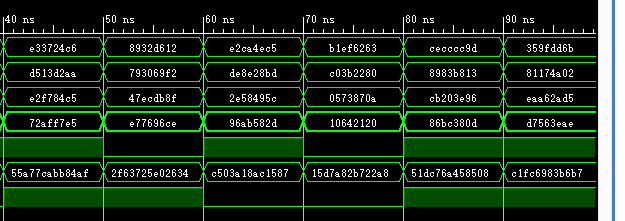
\includegraphics[width=1\textwidth]{./figures/wave.png}
    \caption{实验原理图}
    \label{wave}
\end{figure}

可以观察到,再不同的operand和cin的取值下,cout和result都是正确的。
\subsection{上箱验证}
为了在试验箱上验证我们的代码,我们需要首先修改约束文件。
\begin{verbatim}
//此处代码与指导手册相同,故不再列出
set_property PACKAGE_PIN AC21 [get_ports input_sel1]
set_property PACKAGE_PIN AD24 [get_ports input_sel2]
//此处代码与指导手册相同,故不再列出
set_property IOSTANDARD LVCMOS33 [get_ports input_sel1]
set_property IOSTANDARD LVCMOS33 [get_ports input_sel2]
//此处代码与指导手册相同,故不再列出
\end{verbatim}

随后打开 FPGA 实验板,上电,并将下载线与电脑相连。进行烧写 bit 文件。

随后运行程序验证是否正确。

从图\ref{box}中可以看到 LCD 触摸屏上分别显示了 2 个加数和加法结果,
最右侧的led 灯为向高位的进位,该 led 灯为共阴极的,即输入为 0 是亮,为1 是不亮,
由于当前进位为 0,故 led 灯为亮。
拨码开关最右侧的开关用来选择触摸屏输入的数据为加数1 还是加数 2,
当前该开关置为 1,说明触摸屏输入的 32 位数位加数2。
\begin{figure}[ht]
    \centering
    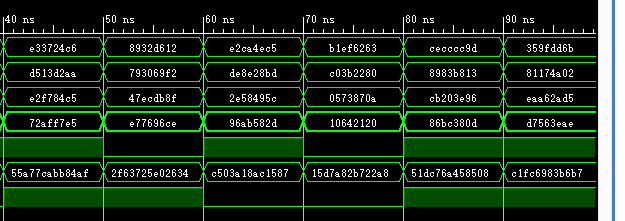
\includegraphics[width=1\textwidth]{./figures/wave.png}
    \caption{实验原理图}
    \label{box}
\end{figure}
\section{实验结果分析}
经过仿真验证和上箱验证,实验结果均符合我的预期,实现了一个64位的加法器模块。
\section{总结感想}
在本次实验中,通过简单的加法器的设计,我基本了解了verilog程序语言设计的流程,包括设计模块,设计仿真文件,以及上箱验证,为以后更困难的计算机组成原理实验打下了基础。

在学习verilog的过程中,我发现它和c语言的语法有许多相似与不相似的地方,于是,我采用对比的方法,更快的完成了对verilog语言的学习。
也体会到了verilog这种硬件描述语言的独特之处。对加法器的原理和设计有了更深的了解,为后续设计cpu的实验打下了基础。
\end{document}